\documentclass[conference]{IEEEtran}
\IEEEoverridecommandlockouts
% The preceding line is only needed to identify funding in the first footnote. If that is unneeded, please comment it out.
\usepackage{cite}
\usepackage{amsmath,amssymb,amsfonts}
\usepackage{algorithmic}
\usepackage{graphicx}
\usepackage{textcomp}
\usepackage{xcolor}
\usepackage{hyperref}
\def\BibTeX{{\rm B\kern-.05em{\sc i\kern-.025em b}\kern-.08em
    T\kern-.1667em\lower.7ex\hbox{E}\kern-.125emX}}
\begin{document}

\title{URL Threat Score Analysis\\
}

\author{\IEEEauthorblockN{ Brandon Julian}
\IEEEauthorblockA{\textit{University of Colorado Boulder} \\
Boulder, United States \\
brju4682@colorado.edu \\
\url{https://github.com/bdjulian/url-threatscore-project}}
}

\maketitle

\begin{abstract}
The Hybrid-Analysis website could possibly be a great resource for dataset creation as the number of threats is extensive (URL, exe, netflows, cmd, etc.). In my attempt to interpret/reverse-engineer Hybrid Analysis™ Falcon Sandbox© incident response threat assessments for malicious URL's; I was successful in determining some feature importances. Using a balance of features that weigh complexity and simplicty I was also successful in rather accurate predictions of Hybrid Analysis URL threat scores on a self created set 200 URL's. Hybrid Analysis's Falcon Sandbox incident response software weighs complexity and verbosity disproportionately compared to other features, and if a URL spawns unnecessary Network Activity it is typically a highly malicious domain. The final model used was a simple Random Forest Regressor tuned by GridSearch and model introspection was done using a variety of methods. If a user wanted to deploy this model they would need to collect their URL traffic information similarly to Hybrid Analysis. The final model proved to be entirely useless as the features it was built on were non-explanatory.
\end{abstract}

\begin{IEEEkeywords}
features, static, dynamic, Network Activity, PDP, SHAP, useful, r2
\end{IEEEkeywords}

\section{Introduction}
As the internet continues to grow, malicious intent also grows with it. The potential for users to be scammed or taken advantage of increases with the ever-evolving attack methods of the unscrupulous. The information and digital security space is an uneven arms race between malicious actors and their victims. By utilizing resources like Hybrid Analysis more tools can be created to help protect ourselves.

\section{Business Understanding}

The goal of this project is to observe what is important in a cutting-edge analysis algorithm of URL's which is otherwise obfuscated as a proprietary product. This modeling process can either be used to deliver on a prediction or inform research and security individuals. By utilizing data already extracted by Hybrid Analysis Falcon Sandbox and constructing it into features for machine learning (ML) it is possible to see what information is most important to an extremely successful product like Falcon Sandbox. If the top features are known it can inform other forensic teams what to look for in their own analysis without needing to deploy a proprietary product. 

\section{Data Understanding}

\subsection{Hybrid Analysis}

To quote their FAQ, “This webpage is a free malware analysis service for the community. Using this service one can submit files for in-depth static and dynamic analysis.”  Files can be submitted to their site for analysis. However, Hybrid Analysis also produces a product they call Falcon Sandbox. Which is a much more verbose system that does most of the dynamic analysis behind the scenes. What is very cool about their website-product integration is when items are submitted for analysis by a user of their product Falcon Sandbox; it by default generates a high-level report of the item in question. This report include interesting features of the item, whether that be signs of attempted access escalation, known malicious artifacts are present, or process spawning. It also includes a threat score out of one-hundred and a final label in the list of malicious, suspicious, no specific threat, no verdict, or whitelisted. The information is stored in two parts - both accessible through their API with a CURL request, a more in-depth explanation on the dataset generation can be found on my \href{https://github.com/bdjulian/url-threatscore-project}{repository}

\subsection{Level of Analysis}
199 total rows were collected. Each row is a URL that has been submitted to the Hybrid Analysis Falcon Sandbox for analysis and assigned a threat score. Any row present in the data has been run through their product by another entity at some point - my data collection range is between the dates of 2020-09-28 and 2020-11-25. This range was chosen for no particular reason other than collection here was more successful than a lot of dates before 2020.

\subsection{Target Variable}

The target for each URL is a continuous number from 0-100 titled 'Threat Score' on the Hybrid Analysis website. All collected URL samples are classified as malicious by Hybrid Analysis intentionally as the intent of the project is to determine what makes something \textit{more dangerous} not necessarily malicious overall.

\subsection{Features}

28 features were created utilizing the Falcon Sandbox reports, the code to create them as well as in-depth explanations of them are on my repository. Brief explanations will be here.

\begin{itemize}
	\item avg-val-length: Average length of value key data in report. Total value divided by number of key value pairs. The value is representative of its type, a payload will have a filename and a hash of the file. While a peristence mechanism will have a registry key and its accompanying value.\\

	\item total-val-len: Total length of value key data.\\

	\item category-count: The number of categories found in the report. A larger category-count means a URL is more complex, possibly possessing multiple types of spawned network activity or multiple methods of payload delivery and installation. The possible unqiue values are: Artifacts Dropped, External Analysis, Network Activity, Payload Delivery, Payload Installation, Persistence Mechanism.\\

	\item Each category type is also a one-hot encoded feature for each row to identify if a malicious URL possesss at least one method, file, or action of the above listed categories. (6 total columns).\\

	\item Each type of category (different from cetegory type) is also one hot encoded: filename-md5, user-agent, domain-ip, mutex, ip-dst, regkey-value, comment, filename-sha512, domain, filename-sha256, link, filename-sha1. (12 total columns)\\

	\item Frequency values were also created form each individual category: this creates 6 more columns for each row which shows how many instances of each category make up the total.\\
\end{itemize}

\begin{figure}[h]
\centerline{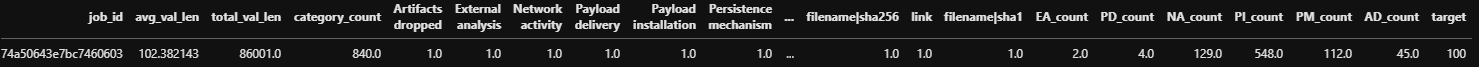
\includegraphics[width=3.5in, height=.2in]{example row.PNG}}
\caption{Example row}
\label{fig}
\end{figure}

\subsection{Descriptive Statistics}
\begin{figure}[h]
\centerline{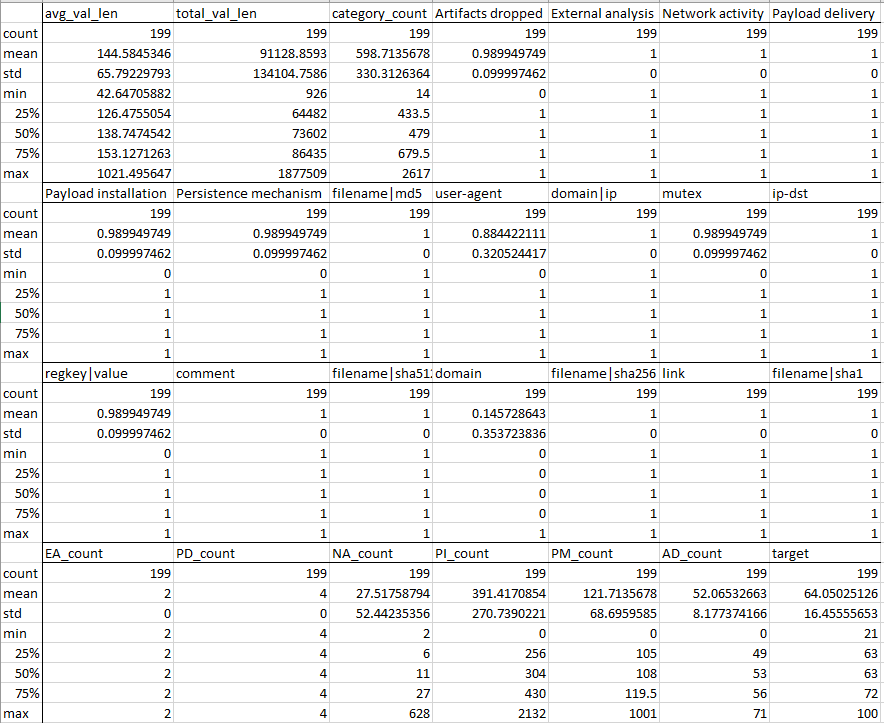
\includegraphics[width=3in, height=4in]{desc-stats.PNG}}
\caption{Descriptive Statistics}
\label{fig}
\end{figure}

Looking at the descriptives of our features. It would appear that in our sample of 199 malicious URL's there is some uniformity of features. Each one-hot column with a minimum of 1 tells us that every observation has that characteristic. For example, each URL has some form of payload delivery or excess network activity. But not all of them possess persistence mechanisms. Our target Threat Score is also skewed towards the max of 100 - however if a malicious URL cannot have a threatscore below 21 (our minimum in the set) that would affect the meaning of these descriptives and visualizations will show this. It would be a good idea to transform these next time. Figures 3 and 4 are visualizations of category-count and our target threat score as well as total-val-len and threat score.These graphs are representative of a few other relaitonships between the target and features. There is typically not an observable linear relationship with some of the most malicious (high threat score) URLS having some of the smaller values of their features. However it is observable that there are almost no occurences of a low threat score URL having a large value in any of the features.
\begin{figure}[h]
\centerline{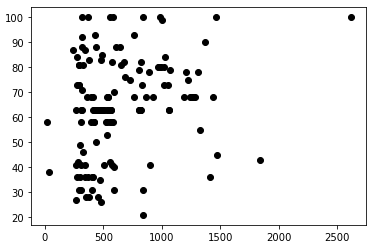
\includegraphics[width=1.5in, height=1.5in]{ts-vs-category.PNG}}
\caption{y = Threat Score, x = category-count}
\label{fig}
\end{figure}
\begin{figure}[h]
\centerline{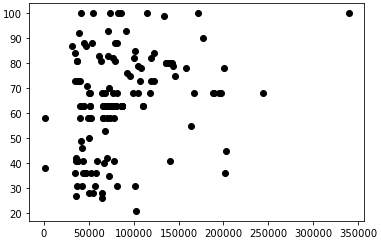
\includegraphics[width=1.5in, height=1.5in]{ts-vs-toalval.PNG}}
\caption{y = Threat Score, x = total-val-len}
\label{fig}
\end{figure}\\

\section{Data Preparation}
\subsection{Data Collection}
Data was collected in two steps using CURL to interact with the Hybrid Analysis API. One collects the job-id and target of a URL submitted on a given day, the other collects the accompanying JSON data used to create the features for each row. Examples of the retrieved data are in my repository.

\subsection{Data Cleaning}
Since there is a large amount of data to choose from it is the analysts pick on how to clean. Instead of doing any true data cleaning for this project the code was written to pass on any data not in the exact format I wanted. If the retrieval failed, pass to the next job-id. If a feature wasn't present - pass to the next job.

\subsection{Feature Engineering}
The information contained in the Falcon Sandbox reports is rich - there are plenty of other features that can be created with it. The majority of the information contained in the reports is generated by dynamic analysis of the URL upon visiting. Falcon Sandbox creates a VM and connects to the submitted URL and captures everything it does to the vulnerable machine. The first CURL request which retrieves the job-id and threatscore also has access to the submitted name of the URL which can be deconstructed into further lexical features. Here are the justifications for each feature I ended up making.\\
\begin{enumerate}
\item avg-val-length: This goes hand in hand with total-val-length. If overall complexity is or is not important that will be captured between the two. By incorporating the average we give weight to URL's that may be dangerous but by only a few extremly dangerous methods.\\
\item total-val-length: This goes hand in hand with avg-val-length. If overall complexity is important this will capture that. Perhaps more complex malicious URL structures are actually more dangerous, or it's structured to try a bunch of weak exploits on its users.\\
\item category-count: This further informs complexity by identifying how many pieces make up the URL's malicious behavior. For instance an entire URL could have just massive registry keys that completely control its total-val-length and avg-val-length. But by counting up the category occurences this will show if a URL is complex by the different pieces it possesses. This may be multiple paylload methods, forms of peristence etc.\\
\item One hot encoded categories: This was a feature intended to shine light on the construction of malicious URL's. The idea was to see if certain pieces were more important in how dangerous a URL was but it instead showed how similar all the URL's in the set were.\\
\item Type of category one-hot encoding: This was another idea to try and identify if certain pieces of the URL's execution were more important that others. But it turned out to be extremely associated with the categories themselves and possessing all types was a pretty homogenous occurence for all URL's.\\
\item Frequency category counts: The purpose here was to further break complexity down. Perhaps a URL with 100 forms of payload delivery, a form of bruteforce attempting to find any exploit in your system would be less dangerous than one that managed to spawn a few instances of uneccessary network activity - exposing you to surveillance or attack from other malicious entities.\\

\end{enumerate}
This is the final feature set available for modeling. However there is plenty of opportunity in the JSON data to create more for other projects, and the lexical analysis is still possible. Known domain generation algorithms (DGA) could also be incorporated to see if Hybrid Analysis draws any analytical importance from that. But in the end the goal of these features is to determine what Hybrid Analysis Falcon Sandbox believes is important, not necessarily what is an important feature in identifying malicious URL's.

\section{Modeling}
My approach to modeling was very simple, I compared two modeling techniques from sklearn. GradientBoostingRegressor and RandomForestRegressor. It is possible lightgbm or xgboost could be implemented for better results. Model introspection is also easier on sklearns own available models. I used a 70-30 random train-test split and used RandomForestRegressors default settings for the first model. I then attempted to optimize the model with GridsearchCV and Recursive Feature Elimination. For model introspection we will observe permutation importance, partial dependence plotting, and SHAP values.
\subsection{Random Forest Regressor}
Using sklearns RandomForestRegressor here is the initial model. And simple performance metrics on the training and testing data.
\begin{figure}[h]
\centerline{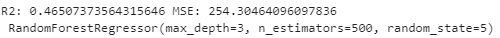
\includegraphics[width=2.75in, height=.25in]{rfrinitial.PNG}}
\caption{RandomForestRegressor training stats}
\label{fig}
\end{figure}
\begin{figure}[h]
\centerline{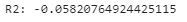
\includegraphics[width=1.5in, height=.125in]{R2test.PNG}}
\caption{RandomForestRegressor test stats}
\label{fig}
\end{figure}
As it turns out, the model is completely uninformative and overfit to the training data. The exact same goes for the GradientBoostingRegressor. Even after parameter optimization with GridsearchCV and recursive feature elimination the model results did not improve. GridsearchCV resulted in the following model (fig 7) and RFE down to 4 features resulted in the following features.\\
\begin{figure}[h]
\centerline{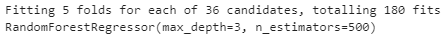
\includegraphics[width=2.75in, height=.25in]{gridsearch.PNG}}
\caption{RandomForestRegressor GridsearchCV}
\label{fig}
\end{figure}
Feature list: avg-val-length, total-val-length, NA-count (network activity), PM-count (persistence mechanism).
On either side, using either modeling technique, the model is either underfit and uninformative or overfit and uninformative.
\section{Evaluation}
Even with the abyssmal results experienced. It could still be of benefit to observe other methods of evalutation. There may still be useful insights in failed experimentation.
\subsection{Permutation Importance}
Besides R2 which is a pretty clear giveaway of model failiure, permuation importance is a very simple way to observe model generalization. Figure 8 shows the permutation importances of the training data and figure 9 shows the importances of the test data. It's obvious with the absolutely massive decrease in importance that there is no model generalization occuring. Whatever the model is learning in the training data is nearly completely unrelatable to the testing data. This is made even more clear with permuation importance after RFE.
\begin{figure}[h]
\centerline{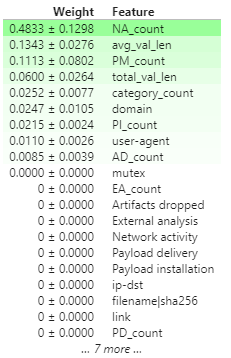
\includegraphics[width=1.75in, height=3.0in]{pitrain.PNG}}
\caption{Permutation Importance Training}
\label{fig}
\end{figure}
\begin{figure}[h]
\centerline{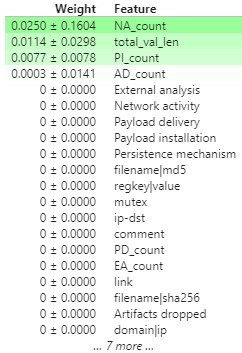
\includegraphics[width=1.75in, height=3.0in]{pitest.PNG}}
\caption{Permutation Importance Test}
\label{fig}
\end{figure}

After runnig RFE to eliminate features down to the top 4 permutation importance again dips in generalization even further. See figure 10. The large decrease in similarity of importances between training and testing (to even negative importance comparison: meaning the model got more accurate in testing when avg-val-len was permuted) just reinforces the idea that the extracted features hold no predictive power over the target variable.

\begin{figure}[h]
\centerline{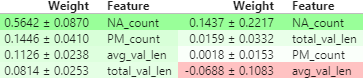
\includegraphics[width=2.75in, height=1.0in]{rfeperm.PNG}}
\caption{Permutation Importance RFE, train left, test right}
\label{fig}
\end{figure}

\subsection{Partial Dependence}
When looking at the partial dependence plots (PDP) we would hope to see any form of relationship between the features and the target. However given the results of the previous evaluation metrics there is a strong chance the PDP will not be informative. We will inspect the top 4 features PDP obtained from RFE.

\begin{figure}[h]
\centerline{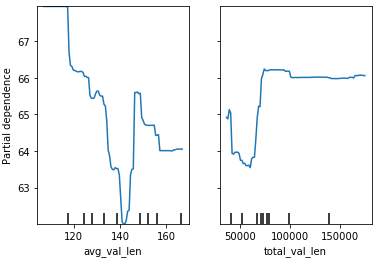
\includegraphics[width=2.75in, height=1.25in]{pdp01.PNG}}
\caption{PDP avg-val-length, total-val-length}
\label{fig}
\end{figure}

As exoected given the other performance metrics. The PDP show that the model is learning weird relationships between the features and the target variable. The PDP for total-val-len looks like it could be learning something useful; however from permutation importance we know this is not the case.

\begin{figure}[h]
\centerline{\includegraphics[width=2.75in, height=1.25in]{pdpna.PNG}}
\caption{PDP PM-count, NA-count}
\label{fig}
\end{figure}

Here is another example (fig 12) of how the model is functioning. As NA (network activity) of a URL increases it will be predicted at a higher threat score, while URL's with more persistence mechanisms will be predicted as lower threat scores. But these insights are only as useful as the model which so far has been determined to be useless so no conclusions should be drawn from the PDP visuals.

\subsection{SHAP Values}

SHAP values are a useful form of model introspection, they can illustrate the individual effects of each feature on a given instance. For simplicities sake since it has already been illustrated that the model holds no predictive value we will quickly look at the RFE model SHAP Values overall and from a small sample. SHAP values hold the same inspection value as PDP as well, they offer insight into how the model itself is using the data provided and what it will do when given an instance with feature vector X. Both PDP and SHAP value analysis should not be used to generalize insights outside of the model - especially in a case such as this where the model has been shown to be not useful.

\begin{figure}[h]
\centerline{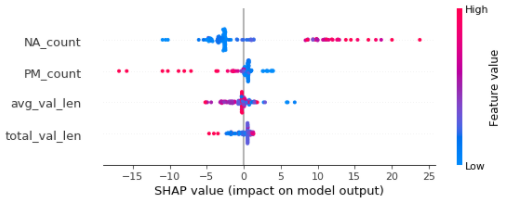
\includegraphics[width=2.75in, height=1.25in]{shapval.PNG}}
\caption{SHAP Values}
\label{fig}
\end{figure}

Figures 14 and 15 are two separate rows from the training data and the model used is the Random Forest Regressor fit to the RFE set.

\begin{figure}[h]
\centerline{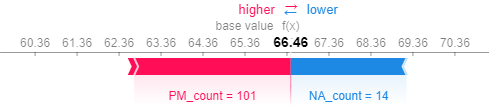
\includegraphics[width=2.75in, height=.75in]{shapsamp1.PNG}}
\caption{Sample 1}
\label{fig}
\end{figure}


\begin{figure}[h]
\centerline{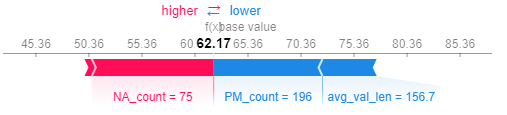
\includegraphics[width=2.75in, height=.75in]{shampsamp2.PNG}}
\caption{Sample 2}
\label{fig}
\end{figure}

Since SHAP considers interaction effects of all the features it's possible in a perfect scenario the values could look like figures 14 and 15 and be completely correct and predictive. Sample 1 has a PM count of 101 which makes it predicted at a higher threat score than the base value and a higher threat score than sample 2 which has a PM count of 196. However what we're seeing here is more realted to what we saw in the PDP for PM-count, as PM-count gets larger the predcited threat score gets lower.\\

Overall the model is proved untrustworthy and should not be used to gain insights into the data other than that this is the wrong feature set to use.

\section{Conclusion}
\subsection{Thoughts}
Sadly the modeling experiemtn was a bust. Yet I still believe the data that can be pulled from Hybrid Analysis's API is extremely useful and this will not be the last time I attempt something like this. I also believe there is also a combination of features that can be created from the JSON data that will be predictive of the threat score. Though it may be the case that Hybrid Analysis is good at protecting their products methods. Even if the methods of Falcon Sandbox cannot be reverse-engineered the data Hybrid Analysis collects is still fantastic. If a URL in the set created excess network activity the contacted domains/ip's were stored alongside the submitted URL. This information can be easily extracted and automated to collate massive blacklists or disover DGA as well.
\subsection{Continued research}
I spent a very long time writing the code for this project so I will not throw it away without another go. I will revisit the feature extraction and find better ways to describe the data. I will also research lexical feature creation and see if that is at all an important feature of Falcon Sandbox analysis.


\end{document}
